% main.tex (20 Nov 2026): official IGARSS 2027 LaTeX template (IEEEtran conference, a4paper).
% TODO: abstract (last, ~150 words), introduction and related work (~350 words, verified references only), conclusion (~70 words), bibliography.
\documentclass[conference,a4paper]{IEEEtran}
\IEEEoverridecommandlockouts
\usepackage[hidelinks]{hyperref}
\usepackage[cmex10]{amsmath}
\usepackage{amssymb,amsfonts}
\usepackage{dblfloatfix}
\usepackage{graphicx}
\usepackage{booktabs}
\usepackage[numbers,compress]{natbib}

\begin{document}

\title{\uppercase{What does a U-Net add? North Indian Ocean subsurface temperature from satellite SST and sea level, checked against a reanalysis and Argo}}

\author{\IEEEauthorblockN{Kanishka Narang}
\IEEEauthorblockA{\textit{Maharaja Agrasen Institute of Technology}\\
New Delhi, India\\
\textbf{[FILL: email]}}}

\maketitle

\begin{abstract}
Satellite sea surface temperature and sea level can be used to estimate subsurface temperature, but how much a deep network adds over simple baselines, and how the answer depends on the reference, is rarely measured under a protocol fixed in advance. We train U-Net ensembles to reproduce the GLORYS12 reanalysis at 15 depths (0--1000~m) over the North Indian Ocean from satellite SST and sea level anomaly, and compare them with climatology, a per-cell linear regression and gradient-boosted trees on three test periods, the last prospective and pre-registered. Against GLORYS12 the ensemble improves on the linear regression in RMSE by 1.8, 2.4 and 4.9\%, with the gain concentrated at 50--200~m; it is worse near the surface and has no practical skill below 300~m. Against Argo profiles the ranking changes: an ensemble variant that is worst against GLORYS12 is the closest learned model, but one constant per depth, fitted on validation Argo, recovers essentially its advantage, so we read it as bias reduction. Intervals cover day-sampling variability only.
\end{abstract}

\begin{IEEEkeywords}
subsurface temperature, U-Net, sea level anomaly, GLORYS12, Argo, North Indian Ocean
\end{IEEEkeywords}

% Introduction v1 (20 Nov 2026). Statements about cited papers are abstract-level only (author has not read the full papers).
% Before submission the author must read each cited abstract and confirm. No novelty claim is made (the IGARSS template asks for one; our rules forbid it).

\section{Introduction}
\label{sec:intro}
Subsurface ocean temperature is observed sparsely, whereas satellite sea surface temperature (SST) and sea level are dense in space and time. Estimating the subsurface from the surface is therefore an established problem, and neural networks are increasingly used for it \cite{smith2023}. Recent studies train networks to estimate temperature, and in some cases salinity, from satellite fields: in the tropical Indian Ocean with Argo data \cite{qi2023}, in the Atlantic from in situ vertical profiles \cite{smith2023}, and in the northwestern Pacific from Argo and ship-based profiles \cite{chae2026} or as daily three-dimensional fields from real-time SST and sea level \cite{wang2026}. These studies propose a network and report how accurate it is against observations or other models.

We ask a different question: how much does a deep network add over strong baselines, and how much of the answer depends on the reference it is scored against? We train U-Nets \cite{unet} to reproduce the GLORYS12 reanalysis \cite{glorys12} at 15 depths from 0 to 1000~m over the North Indian Ocean, using only SST \cite{ostia} and sea level anomaly \cite{duacs} as inputs. We compare them with seasonal climatology, a per-cell linear regression and gradient-boosted trees \cite{xgboost} under a protocol fixed before any test period was opened: chronological splits, three test periods, the last of them prospective and pre-registered, and block-bootstrap intervals for every difference. We also score every estimate against Argo profiles. Argo is assimilated by GLORYS12, so the two references are not independent, and we do not present them as such.

This paper makes three contributions. (i)~It measures the gain of a U-Net ensemble over a linear regression against GLORYS12 on three periods, and shows where the gain appears (the thermocline) and where it does not (near the surface and below 300~m). (ii)~It shows that the ranking of models depends on the reference: an ensemble variant that is worst against GLORYS12 is closest to Argo, and a single constant per depth, fitted on validation Argo, recovers essentially the whole difference. (iii)~It states which analyses were pre-registered and which were specified after the test periods were scored. We claim neither real-time use nor skill below 300~m. Section~\ref{sec:data} describes the data and methods, Section~\ref{sec:results} the results and Section~\ref{sec:discussion} their limits.


% Data and Method v2 (20 Nov 2026). Values checked against configs/*.yaml and scripts (splits, training schedule, XGBoost settings, demeaning).
% TODO fill: Argo GDAC access date and DOI for the earlier months. TODO: all \cite keys must be verified by the author with DOIs.

\section{Data and method}
\label{sec:data}
\emph{Data.} All fields are on a daily $0.25^\circ$ grid over $45$--$105^\circ$E and $5$--$30^\circ$N ($101\times241$ cells). The target is GLORYS12 potential temperature \cite{glorys12} at 15 depths from 0 to 1000~m (0, 5, 10, 20, 30, 50, 75, 100, 125, 150, 200, 300, 500, 700 and 1000~m). The inputs are OSTIA reprocessed SST (v202003) \cite{ostia} and DUACS multi-mission sea level anomaly (SLA, v202411) \cite{duacs}. Of the 12,038 ocean cells, 9,140 are valid at all 15 depths (the \emph{deep set}); every headline number uses this set. From July 2021 GLORYS12 is the interim production of the same product (\texttt{cmems\_mod\_glo\_phy\_my\_0.083deg\_P1D-m}, v202311), so Tests~B and C use an interim target.

\emph{Protocol.} Splits are chronological: training 2010-02-04 to 2017-12-31; validation 2018-02-01 to 2020-01-31 (widened from one year on 25 October 2026, before any model was trained); Test~A 2020-03-02 to 2021-06-27; Test~B 2021-08-01 to 2025-12-31; and Test~C 2026-01-01 to 2026-05-15 (135 days). Gaps between training, validation, Test~A and Test~B are at least 30 days; Test~C follows Test~B directly. Test~C is prospective: its protocol and four predictions were committed on 15 November 2026 (commit 9869230) before any 2026 file was downloaded, although the 2026 data existed publicly before the models were frozen. All models were frozen before any test period was opened. Each test period was scored once under a lock file; the only reruns were for code or output fixes and were logged, including an Argo scoring of Test~C that returned no rows because the profile-pair file lacked 2026 profiles.

\emph{Argo.} Delayed-mode and adjusted Argo profiles are matched to the nearest $0.25^\circ$ cell and day, converted to potential temperature with TEOS-10 \cite{teos10}, and compared at the same cell, day and depth with every estimate and with GLORYS12; 0~m is dropped. The 2026 profiles were downloaded on 16 November 2026 through argopy \textbf{[FILL: access date and DOI for the earlier months]}; Test~C has 507 such profiles. Argo is assimilated by GLORYS12, so it is not independent of the target.

\emph{Models.} Inputs and targets are anomalies relative to a per-cell harmonic seasonal cycle (three harmonics) fitted on training days only; inputs are divided by training standard deviations, and the network predicts the target anomaly (scaled by 2). The U-Net \cite{unet} has width 32 and about 0.47 million parameters. It maps SST and SLA anomalies and an ocean mask to 15 anomaly maps and has no season input. Training used AdamW (learning rate $10^{-3}$, weight decay $10^{-4}$), cosine annealing over at most 25 epochs, batch size 8, every second training day (1,444 days) and early stopping on the validation loss (patience 6). The \emph{frozen ensemble} averages six U-Nets: three seeds with same-day inputs and three with inputs at lags of 0, 7, 14 and 30 days. The \emph{demeaned ensemble} is identical except that the daily deep-set mean of SLA is removed before standardisation; it was pre-registered as co-primary and is always reported.

\emph{Baselines.} (i)~Seasonal climatology. (ii)~A per-cell, per-depth linear regression on the SST and SLA anomalies. (iii)~XGBoost \cite{xgboost}, one model per depth, with the two anomalies, latitude, longitude and the sine and cosine of the day of year as features and fixed untuned settings (300 trees, learning rate 0.05, depth 6), fitted on every tenth training day and 1,500 random deep-set cells per day; it covers the deep set only. (iv)~A single U-Net (seed 0), which is the first member of the frozen ensemble. All are fitted on training days only.

\emph{Argo-calibrated correction.} For each of the 14 Argo depth levels, the mean of (estimate minus Argo) over validation-window profiles is subtracted from the estimate at every cell and day: one constant per depth, fitted on validation Argo only. The rule was pre-registered (commit 035f117) after the test periods had been scored, so it is pre-specified but not blind. Its extension to all estimates (commit 3d1ed25) and the comparison of XGBoost and the ensemble by season are exploratory.

\emph{Metrics.} Against GLORYS12, pooled RMSE is the square root of the mean over the 15 depths of the per-depth MSE on the deep set. Against Argo it is the RMSE over all matched profile-depth values at 14 levels, on the rows where every estimate is finite. Intervals for paired RMSE differences use a moving-block bootstrap over days (30-day blocks, 2,000 resamples); they reflect day-sampling variability, not training randomness, and Test~C contains about 4.5 blocks.

% Results v2 (19 Nov 2026). Every number comes from docs/results_ledger.md or paper/tables/tab_main.tex (generated and
% cross-checked by scripts/make_results_table.py). The old results.tex is kept for reference. Do not retype numbers from memory.

\section{Results}
\label{sec:results}

\begin{table*}[t]
\centering
\caption{Pooled RMSE ($^\circ$C) on the deep set. Against GLORYS: mean of the per-depth MSE over 15 depths. Against Argo: all matched profile-depth values at 14 levels (5--1000~m), equally weighted ($48522$, $139583$ and $6895$ values in Tests~A, B and C; Test~C has 507 profiles). The two pooling rules are not comparable in magnitude. Corrected: one additive constant per depth, fitted on validation-window Argo only. Argo is assimilated by GLORYS and is not independent of it. In the corrected columns the GLORYS12 row is GLORYS12 with its own per-depth constants applied. Best learned model in bold per column (GLORYS12 and climatology excluded).}
\label{tab:main}
\begin{tabular}{@{}lccccccccc@{}}
\hline
 & \multicolumn{3}{c}{vs GLORYS} & \multicolumn{3}{c}{vs Argo, raw} & \multicolumn{3}{c}{vs Argo, corrected} \\
\cline{2-4}\cline{5-7}\cline{8-10}
Model & A & B & C & A & B & C & A & B & C \\
\hline
Climatology & 0.969 & 1.068 & 0.906 & 1.009 & 1.106 & 0.817 & -- & -- & -- \\
Linear (SLA+SST) & 0.683 & 0.746 & 0.670 & 0.861 & 0.932 & 0.831 & 0.782 & 0.869 & 0.697 \\
XGBoost & 0.682 & 0.741 & 0.639 & 0.855 & 0.920 & 0.777 & 0.779 & 0.863 & 0.668 \\
Single U-Net & 0.690 & 0.745 & 0.642 & 0.848 & 0.917 & 0.779 & 0.776 & 0.864 & 0.668 \\
U-Net ensemble & \textbf{0.671} & \textbf{0.728} & \textbf{0.637} & 0.834 & 0.909 & 0.773 & \textbf{0.757} & \textbf{0.843} & \textbf{0.661} \\
Ensemble, demeaned SLA & 0.743 & 0.810 & 0.705 & \textbf{0.754} & \textbf{0.848} & \textbf{0.649} & 0.791 & 0.879 & 0.698 \\
\hline
GLORYS12 & -- & -- & -- & 0.677 & 0.783 & 0.711 & 0.641 & 0.735 & 0.668 \\
\hline
\end{tabular}
\end{table*}


\subsection{Agreement with GLORYS}
Against GLORYS, the frozen ensemble has a pooled deep-set RMSE of 0.671, 0.728 and 0.637$^\circ$C on Tests~A, B and C (Table~\ref{tab:main}), against 0.683, 0.746 and 0.670$^\circ$C for the per-cell linear regression and 0.969, 1.068 and 0.906$^\circ$C for the seasonal climatology. Its gain over the linear regression is $-1.8\%$ (95\% interval $[-2.9,-0.7]$), $-2.4\%$ ($[-3.2,-1.6]$) and $-4.9\%$ ($[-7.2,-3.0]$). The pre-registered prediction for the prospective Test~C, a gain of a few percent at most, held in direction, but the gain is about twice that of Tests~A and B. Over XGBoost the gain is $-1.6\%$ ($[-2.9,-0.5]$) and $-1.7\%$ ($[-2.6,-0.9]$) on Tests~A and B, and a tie on Test~C ($-0.3\%$, $[-1.7,+1.8]$).

\begin{figure*}[t]
\centering
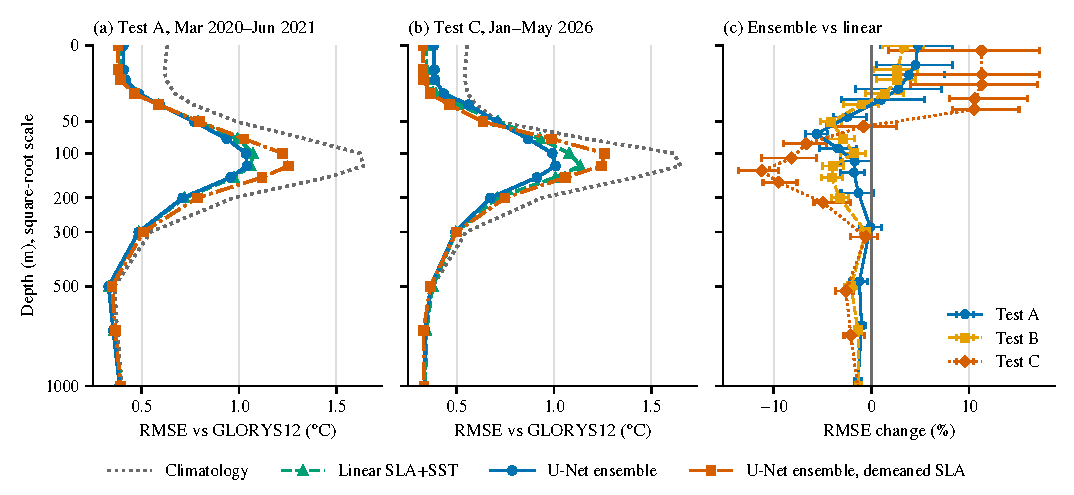
\includegraphics[width=\textwidth]{figures/fig_rmse_by_depth_v2.pdf}
\caption{(a)~RMSE against GLORYS12 by depth on the deep set for Test~A and (b)~for Test~C. (c)~RMSE change of the U-Net ensemble relative to the linear regression with 95\% block-bootstrap intervals for Tests~A, B and C (negative is better; Test~B is shown only here); points are offset vertically for legibility. The depth axis is a square-root scale.}
\label{fig:depth}
\end{figure*}

The gain is concentrated in the thermocline (Fig.~\ref{fig:depth}): at 50--200~m it is $-2.8\%$, $-3.2\%$ and $-7.9\%$ ($[-9.8,-6.2]$ on Test~C). Near the surface the ensemble is worse than the linear regression, by $2.7$--$4.8\%$ at 0--10~m on Tests~A and B (at most $0.02^\circ$C) and by $10.9\%$ ($[+6.2,+15.8]$) at 0--30~m on Test~C. Below 300~m the gains are at most about $0.01^\circ$C ($-1.5\%$, $[-2.3,-0.6]$, on Test~C), and we do not count them as skill. The demeaned ensemble, pre-registered as co-primary, is $10.7$--$11.2\%$ worse than the frozen ensemble against GLORYS in all three periods.

\subsection{Agreement with Argo profiles}
Against Argo, GLORYS itself has an RMSE of 0.677, 0.783 and 0.711$^\circ$C, and the frozen ensemble 0.834, 0.909 and 0.773$^\circ$C (Table~\ref{tab:main}). The ensemble is closer to Argo than the linear regression by $3.1\%$ ($[-5.3,-1.3]$), $2.5\%$ ($[-3.8,-1.3]$) and $7.0\%$ ($[-10.9,-3.5]$), but only at 75--200~m ($-5.5\%$, $-5.5\%$, $-10.3\%$); at 5--50~m it is worse ($+3.8\%$, $+2.7\%$, $+8.8\%$). The ranking of the two ensembles reverses with the reference: the demeaned ensemble is the closest learned model to Argo, by $9.7\%$ ($[-12.8,-7.7]$), $6.7\%$ ($[-8.5,-4.9]$) and $16.1\%$ ($[-20.1,-14.4]$) relative to the frozen ensemble. On Test~C its RMSE (0.649$^\circ$C) is below that of GLORYS, which we do not read as better than GLORYS: the period covers one season, with 507 profiles, and the reason below applies.

The reason is bias, not pattern. In the thermocline (75--200~m) the models inherit the warm bias of GLORYS relative to Argo (on Test~C: GLORYS $+0.403$, frozen $+0.607$, linear $+0.771^\circ$C). After removing each year's mean bias (2018--2025), the demeaned and frozen ensembles have the same RMSE (1.024 and 1.026$^\circ$C), so the demeaned advantage is a bias reduction; its yearly bias changes sign.

\subsection{A bias correction against Argo}
We therefore tested the simplest remedy. For each depth we subtract one constant, the mean model-minus-Argo difference on the validation-window Argo profiles (up to $0.51^\circ$C at 100--125~m), from every prediction. This analysis was specified in a pre-registration after the test periods had been scored (pre-specified, not blind), and uses no test data to fit anything. Its success rule was met: the corrected frozen ensemble is closer to Argo than the uncorrected one by $9.3\%$ ($[-11.8,-7.8]$), $7.2\%$ ($[-8.4,-6.2]$) and $14.6\%$ ($[-16.3,-14.1]$) on Tests~A, B and C, at the cost of agreement with GLORYS (0.671 to 0.716, 0.728 to 0.785 and 0.637 to 0.649$^\circ$C).

One pre-registered prediction failed: P2 expected the correction to help less than the demeaned ensemble does. Against the uncorrected demeaned ensemble, the corrected frozen ensemble differs by $+0.4\%$ ($[-0.5,+1.5]$), $-0.6\%$ ($[-2.2,+0.8]$) and $+1.9\%$ ($[+0.1,+4.9]$): one constant per depth recovers essentially the whole demeaned advantage against Argo. The correction is standard practice and is not offered as a method.

As an exploratory check, chosen after seeing these results, we applied the same rule to every estimate. The correction improves the linear regression by $9.1\%$, $6.8\%$ and $16.1\%$ and GLORYS by $5.3\%$, $6.1\%$ and $6.0\%$. The corrected ensemble stays ahead of the corrected linear regression ($-3.2\%$, $-2.9\%$, $-5.2\%$; at 75--200~m $-4.7\%$, $-5.5\%$, $-7.3\%$) and, by less, of corrected XGBoost ($-2.9\%$, $-2.2\%$, and $-1.1\%$ with interval $[-3.0,+0.5]$ on Test~C) and of the corrected single U-Net ($-2.4\%$, $-2.4\%$, $-1.1\%$). The near-surface deficit disappears, so it was bias: at 5--50~m the corrected ensemble ties the corrected linear regression in all three periods. Corrected GLORYS remains closer to Argo than the corrected ensemble on Tests~A and B ($+18.0\%$ and $+14.7\%$), with a tie on Test~C ($-1.1\%$, $[-6.7,+6.7]$).

\subsection{Further observations}
Exploratory and not pre-registered: XGBoost, which receives the day of year, was better than the ensemble at 30--50~m in January--May of six of seven years (point estimates; $+19.2\%$ at 30~m and $+22.1\%$ at 50~m in 2026, with a reversal in 2024); we do not claim a cause. Against GLORYS, among the Arabian Sea, Bay of Bengal and Andaman Sea, only the Bay of Bengal shows a gain over the linear regression with intervals excluding zero in both Test~A and Test~B ($-5.6\%$, $-3.8\%$); the validation-window advantage in the Andaman Sea ($-12.5\%$) did not replicate. Integrated Gradients on 19 validation days show reliance on SST near the surface (share 0.63 at 0~m) and on sea level at depth (0.72 at 50~m, 0.84 at 150~m); this is reliance, not correctness.

% Discussion v2 (20 Nov 2026). Every statement is backed by docs/results_ledger.md. Conclusion (about 70 words) still to write.

\section{Discussion and limitations}
\label{sec:discussion}
Sea surface temperature and sea level let a per-cell linear regression remove much of the climatological error; the U-Net ensemble adds a further $1.8$ to $4.9\%$ against GLORYS12, almost all at 50--200~m, and nothing useful near the surface or below 300~m. We read this as a measurement of what a deep network adds beyond a linear baseline under a protocol fixed before the test years, not as an accuracy record.

The reference matters more. The estimates are trained on GLORYS12, which is warmer than Argo in the thermocline, and they inherit the offset. The demeaned ensemble ranks last against GLORYS12 and first among the learned models against Argo, but one constant per depth, fitted on validation-window Argo, gives the frozen ensemble nearly the same Argo gain, so we read the demeaned advantage as bias reduction. The constants improve the frozen ensemble, the linear regression and GLORYS12 itself (by 5--6\%), but not the demeaned ensemble, which was already bias-reduced; the frozen ensemble keeps a smaller advantage of 3--5\% over the corrected linear regression. XGBoost, which receives the day of year, was better than the ensemble at 30--50~m in January--May of six of seven years (point estimates, no intervals); a season input is a hypothesis we did not test.

\emph{Limitations.} (i)~The target is a reanalysis that assimilates Argo, so the Argo comparison is not independent. (ii)~Intervals cover day-sampling variability only; Test~C is one season, 135 days (about 4.5 blocks) and 507 profiles. (iii)~The correction, its extension and the XGBoost analysis were specified after the test periods had been scored. (iv)~The single U-Net is a member of the ensemble, and the Andaman Sea advantage seen in validation did not replicate. (v)~Tests~B and C use interim GLORYS12; one domain, one reanalysis.


\section{Conclusion}
\label{sec:conclusion}
Under a frozen protocol, a U-Net ensemble driven by satellite SST and sea level improves on a per-cell linear regression by 1.8 to 4.9\% against GLORYS12, mostly in the thermocline. The reference matters more: against Argo the ordering of two ensembles reverses, by 6.7 to 16.1\%, through a bias that one constant per depth largely reproduces. Estimates trained on a reanalysis should be checked against profiles, and gains reported with intervals. We claim neither real-time use nor skill below 300~m.

\small
\bibliographystyle{IEEEtranN}
\bibliography{references}

\end{document}
